\PassOptionsToPackage{unicode}{hyperref} 
\documentclass{beamer}

% --- Налаштування мови та шрифтів ---
\usepackage[T2A]{fontenc}
\usepackage[utf8]{inputenc}
\usepackage[ukrainian]{babel}
\usepackage{graphicx}

% Фікс для математичних шрифтів та чіткості
\usefonttheme[onlymath]{serif} 

% --- ТЕМА ТА КОЛЬОРИ ---
\usetheme{CambridgeUS}
\usecolortheme{dolphin} 

% --- НАЛАШТУВАННЯ ЯСКРАВОСТІ РАМОК (БЛОКІВ) ---
\setbeamercolor{block title}{fg=white, bg=blue!80!black}
\setbeamercolor{block body}{fg=black, bg=blue!10}
\setbeamercolor{block title example}{fg=white, bg=green!50!black}
\setbeamercolor{block body example}{fg=black, bg=green!10}
\setbeamercolor{block title alert}{fg=white, bg=red!70!black}
\setbeamercolor{block body alert}{fg=black, bg=red!10}

\setbeamercolor{normal text}{fg=black}
\setbeamerfont{block title}{series=\bfseries}

% --- НАЛАШТУВАННЯ ПІДПИСІВ ---
\setbeamertemplate{caption}[numbered] 
\setbeamertemplate{caption label separator}{. } 
\addto\captionsukrainian{\renewcommand{\figurename}{Рис.}}

% --- ДАНІ ТИТУЛЬНОГО СЛАЙДА 
% У квадратних дужках [...] пишіть коротко, у фігурних {...} — повно
\title[Теорема Піфагора]{Застосування теореми Піфагора}
\subtitle{Трикутник та його види}
\author[Прізвище І.П.]{ Бондар Наталія Вікторівна}
\institute[ФМФ]{Факультет математики, фізики та комп'ютерних наук}
\date{\today}

\begin{document}

% 1. ТИТУЛ
\begin{frame}
\titlepage
\end{frame}

% 2. ЗМІСТ
\begin{frame}{План}
\tableofcontents
\end{frame}

% 3. ТРИКУТНИК
\section{Трикутник}

\begin{frame}{Що таке трикутник?}
Трикутник — це геометрична фігура, яка має:
\begin{itemize}
    \item 3 сторони
    \item 3 вершини
    \item 3 кути
\end{itemize}
\end{frame}

% 4. ВИДИ ЗА СТОРОНАМИ
\section{Види трикутників за сторонами}

\begin{frame}{Види за сторонами}

\begin{block}{Рівносторонній}
Усі сторони рівні.
\end{block}

\begin{block}{Рівнобедрений}
Дві сторони рівні.
\end{block}

\begin{block}{Різносторонній}
Усі сторони різні.
\end{block}

\end{frame}

% 5. ВИДИ ЗА КУТАМИ
\section{Види за кутами}

\begin{frame}{Види трикутників за кутами}

\begin{columns}

\begin{column}{0.5\textwidth}
\begin{itemize}
    \item Гострокутний ($<90^\circ$)
    \item Прямокутний ($=90^\circ$)
    \item Тупокутний ($>90^\circ$)
\end{itemize}
\end{column}

\begin{column}{0.5\textwidth}
\centering
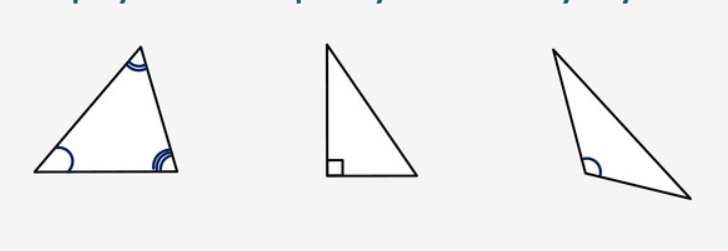
\includegraphics[width=\textwidth]{FOTO1}
\end{column}

\end{columns}

\end{frame}

% 6. СУМА КУТІВ
\section{Властивості трикутника}

\begin{frame}{Сума кутів}

\begin{block}{Властивість}
Сума кутів будь-якого трикутника:
\[180^\circ\]
\end{block}

\end{frame}

% 7. ПІФАГОР
\begin{frame}{Теорема Піфагора}

\begin{columns}

\begin{column}{0.5\textwidth}
Для прямокутного трикутника:

\[a^2 + b^2 = c^2\]

\begin{itemize}
    \item $a, b$ — катети
    \item $c$ — гіпотенуза
\end{itemize}

\vspace{0.3cm}

\textbf{Приклад:}
\[3^2 + 4^2 = 5^2\]

\[9 + 16 = 25\]

\end{column}

\begin{column}{0.5\textwidth}
\centering
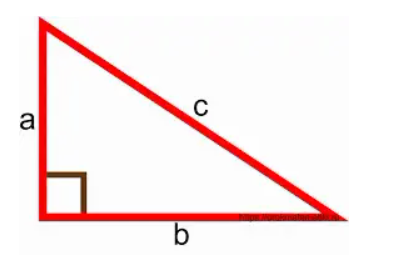
\includegraphics[width=0.9\textwidth]{FOTO2}
\end{column}

\end{columns}

\end{frame}

% --- ПЕРИМЕТР ТРИКУТНИКА ---
\begin{frame}{Периметр трикутника}

\begin{block}{Визначення}
Периметр трикутника — це сума довжин усіх його сторін.
\end{block}

\[P = a + b + c\]

\vspace{0.5cm}

\textbf{Приклад:}

\[P = 3 + 4 + 5 = 12\]

\end{frame}

% 8. ЗАСТОСУВАННЯ
\section{Застосування}

\begin{frame}{Де використовується}

\begin{enumerate}
    \item Будівництво та архітектура
    \item Картографія та навігація
    \item Інженерія
    \item Фізика
\end{enumerate}

\end{frame}

% 9. ВИСНОВОК
\begin{frame}{Висновок}

\centering
\Large
Трикутники та теорема Піфагора  
є основою геометрії та практичних обчислень.

\vspace{1cm}

\textbf{Дякую за увагу!}

\end{frame}

\end{document}
